\documentclass[a4paper,10pt]{report}
\usepackage[utf8]{inputenc}

% Title Page
\title{Um Modelo Convolucional Capaz de Realizar a Predição para Valores da Função Seno}
\author{Isaac L. S. Sacramento}


\begin{document}
\maketitle

\begin{abstract}
\end{abstract}

\chapter{Introdução}

As Redes Neurais Convolucionais são amplamente utilizadas
na solução de problemas cujo objetivo é classificar elementos
dentro de um determinado domínio. Diversos modelos de redes
convolucionais surgem a cada dia para resolver problemas específicos
de classificação como.

Por outro lado há domínios em que um conjunto de imagens representa
um fenômeno espacialmente distribuído. Exemplos de fenômenos 
espacialmente distribuídos são: eventos geoestatísticos como 

Neste tipo de evento, os pontos da imagem estão espacialmente correlacionados,
de modo que para realizar um estudo sobre este tipo de evento, é
importante levar em consideração esta correlação. A correlação é dada
pela fórmula X, de modo que pontos espacialmente próximos estão mais fortemente
correlacionados do que pontos espacialmente distantes.

Quando os métodos baseados em redes neurais tradicionais são utilizados
para lidar com problemas relacionados a fenômenos espacialmente distribuídos
a informação de correlção espacial costuma ser perdida, uma vez que as imagens
são tratadas como vetores na entrada da rede, de modo que não há interpretação
da correlação espacial. Por outro lado,

\chapter{Redes Neurais Convolucionais Regressivas}

\section{Predição da Função Seno}
O uso da função seno como experimento inicial visa alcançar um modelo de
rede convolucional capaz de realizar a aproximação de função utilizando
imagens da função. A função seno foi arbitrariamente escolhida para
representar um conjunto de treinamento não-linear, mas ainda simples o
suficiente que permitisse obter um modelo convolucional capaz de realizar predição
ao invés de classificação. É importante ressaltar que este modelo deve ser
aprimorado e adaptado para a resolução de problemas com conjuntos de dados
do mundo real.

%For training shallow neural networks it is commonly used the input values for
%sin function in the interval $-\pi , \pi$. 
\subsection{Conjunto de Dados}
O conjunto de treinamento das redes neurais convencionais é geralmente composto
pelos valores das propriedades de entrada e os valores da propriedade que se
deseja prever. Para prever a função seno com redes neurais convencionais, o
conjunto de entrada compreende valores $x$ no intervalo [$-k\pi,k\pi$],
$k >= 1$. Tendo em vista que o conjunto de entrada das redes neurais convolucionais
são imagens de treinamento a partir das quais se deseja extrais padrões espaciais
que permitam realizar predição, para este primeiro experimento foi gerada uma
matriz de senos. Nesta matriz de senos, cada linha representa uma imagem em 1D
composta por $10$ valores subsequentes da função seno, o valor seguinte é o que se
deseja prever. A Figura \ref{} ilustra a forma como o conjunto experimental de imagens
de treinamento foi gerado. É importante salientar que, neste caso os valores dos ângulos de entrada para a função
seno não são utilizados como entrada da rede convolucional, de modo que a predição
deverá ocorrer baseada no entendimento do padrão da curva existente no conjunto de
de $10$ valores da função. Todo o conjunto é inicialmente por $90$ imagens.

\begin{figure}[htp]
\begin{center}
  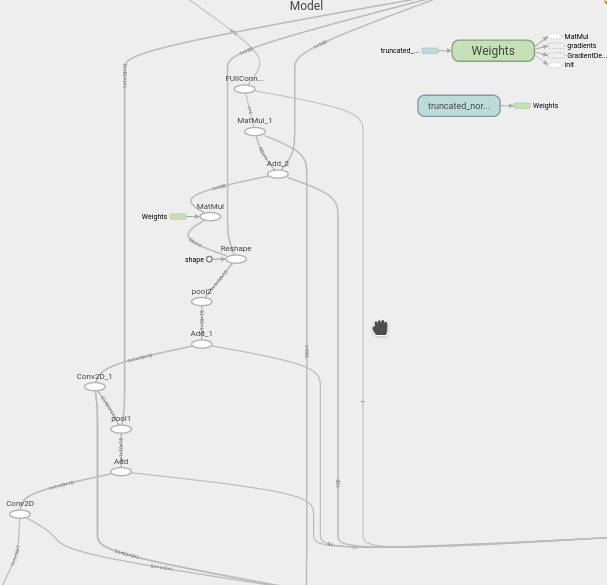
\includegraphics[width=0.7\textwidth]{cnn_model}
  \caption{Conjunto de imagens de treinamento para a função seno.}
  \label{fig:sinFunc}
\end{center}
\end{figure}

\subsection{Parâmetros do Modelo}
O estudo de sensibilidade dos hiper-parâmetros do modelo convolucional objetivou 
alcançar uma configuração capaz de realizar a predição da função seno.
Nesta seção são listados os parâmetros estudados, os quais foi testados
para diferentes valores e combinações entre eles.

 \begin{description}
   \item[Função de Custo] fruta amarela, a forma lembra a Lua.
   \item[Número d] fruta vermelha e arredondada.
 \end{description}
  

\subsection{Modelo Convolucional}
O modelo de rede neural convolucional apresentado neste trabalho
emergiu de forma incremental e permitiu um melhor
entendimento do potêncial de uso do funcionamento da biblioteca.
Inicialmente foram testados diferentes modelo mais simples composto
por uma camada convolucional, uma camada de \textit{pooling},
uma camada completamente conectada e, por fim, um neurônio de saída.
Este modelo é ilustrado na Figura \ref{}. Por meio deste modelo
prévio foi possível realizar um estudo de sensibilidade de cada um
dos parâmetros do modelo, bem como de cada uma das funções de
ativação disponibilizadas na biblioteca.

\begin{figure}[htp]
\begin{center}
  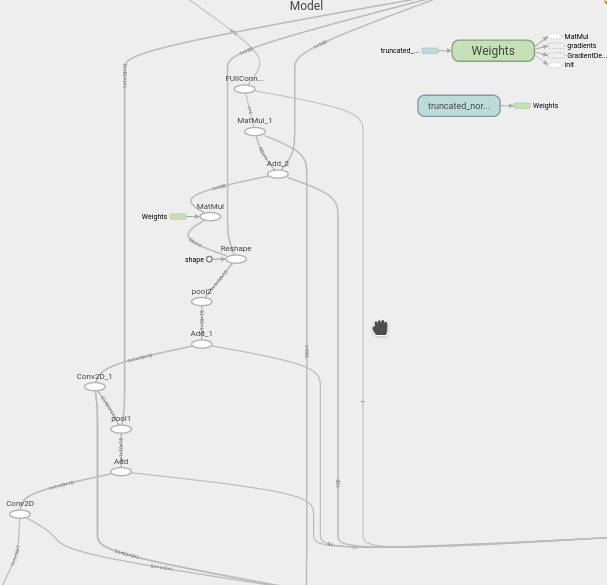
\includegraphics[width=0.7\textwidth]{cnn_model}
  \caption{Modelo de RNC simplificado inicial}
  \label{fig:rncSimple}
\end{center}
\end{figure}

O modelo que apresentou maior estabilidade na predição dos valores
da função seno é ilustrado na Figura \ref{}. Este modelo segue a
estrutura básica para as redes neurais convolucionais e é composto
por duas camadas convolucionais, cada uma das quais é seguida por uma
camada de pooling, uma camada completamente conectatada e um
neurônio na camada de saída.

\begin{figure}[htp]
\begin{center}
  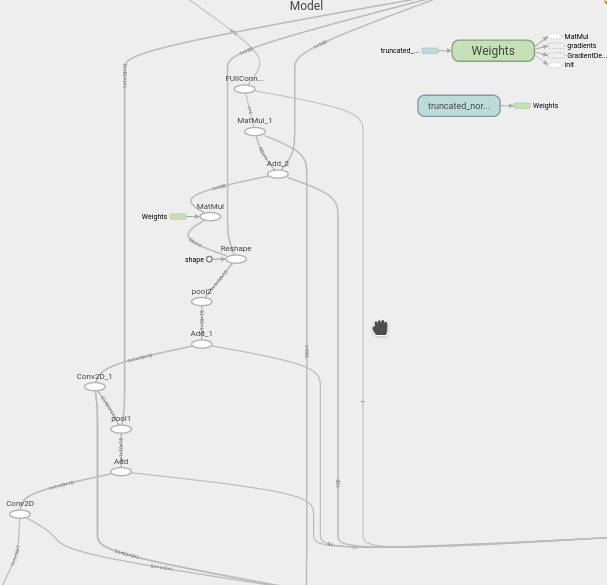
\includegraphics[width=0.7\textwidth]{cnn_model}
  \caption{Modelo de RNC simplificado para predição da função seno.}
  \label{fig:rncComplete}
\end{center}
\end{figure}

\end{document}          
